%% --------------------------------------------------------------
%%
%% A F T E R G L O W
%%
%% --------------------------------------------------------------
\begin{frame}{Introduction}
\begin{tikzpicture}[overlay,remember picture]
\uncover<1->{ % <-> |
    \node (t1) [anchor=center,scale=1,opacity=1] at ([shift={(-2.9cm,1.3cm)}]current page.center){
        \parbox{0.70\textwidth}{
            GRBs, cocoon, ejecta produce afterglow \\
            Synchrotron emission arising when a shock propagates through ISM
            \begin{itemize}
            \item Trace physics of jet formation
            \item Information on the fastest ejecta
            \end{itemize}
    }};
}

\uncover<1->{ % <-> |
    \node (t1) [anchor=center,scale=1,opacity=1] at ([shift={(-2.9cm,-2.0cm)}]current page.center){
        \parbox{0.70\textwidth}{
            \GRB{}, non-thermal EM counterpart to \GW{}
            \begin{itemize}
            \item Very long follow-up
            \item Structured jet model explans slow rise
            \item Spectrums is described by power law$^{(*)}$
            \end{itemize}
    }};
}

%\uncover<1->{ % <-> |
%    \node (t1) [anchor=center,scale=1,opacity=1] at ([shift={(-3.6cm,-3.5cm)}]current page.center){
%        \parbox{0.60\textwidth}{
%            Several open questions
%            \begin{itemize}
%            \item Insufficient ejecta to explain early blue part.
%            \end{itemize}
%    }};
%}

\uncover<1->{ % <-> |
    \node (img1) [anchor=center,scale=1,opacity=1] at ([shift={(6.0cm,-0.8cm)}]current page.center){
        \parbox{0.5\textwidth}{
            \includegraphics[height=6.3cm]{jet_ascenci20.pdf}

            Artist depiction of ejecta$^\text{\citep{Ascenzi:2020xqi}}$
    }};
}
\end{tikzpicture}
\end{frame}

%% =======================================================
%%
%%                   Method
%%
%% =======================================================

\begin{frame}{Method} %% ---------- title 

\begin{tikzpicture}[overlay,remember picture]

\uncover<1->{ % <-> |
    \node (t1) [anchor=center,scale=1,opacity=1] at ([shift={(-3.9cm,-0.7cm)}]current page.center){
        \parbox{0.53\textwidth}{
            Passing through the cold ISM, shock front 
            \begin{itemize}
                \item randomizes the particles' $\vec{\upsilon}$,
                \item compresses the plasma,
                \item amplifies the magnetic fields 
                \item accelerates the inbound particles % to a power-law distribution function.
            \end{itemize}
            
            \textbf{Dynamics} --
            %A relativistic shock propagating into a cold upstream medium.
            $3$ conservation laws: baryon number, energy, momentum fluxes across shock front.
%            The latter two $T^{\mu\nu} = (\rho' c^2 + p') u^{\mu} u^{\nu} + p' g^{\mu\nu},$
            %
%            These equations can be written as 
            %
%            \begin{equation} % subequations
%            \begin{aligned} % align
%            \frac{e_2'}{n_2'} &= (\gamma_{21} - 1)m_p c^2 \\
%            \frac{n_2'}{n_1'} &= \frac{\hat{\gamma}\gamma_{21} + 1}{\hat{\gamma}-1} \\
%            \gamma_{1s}^2 &= \frac{(\gamma_{21} + 1) [\hat{\gamma}(\gamma_{21}-1)+1]^2}{\hat{\gamma}(2-\hat{\gamma})(\gamma_{21}-1)+2}
%            \end{aligned} % align
%            \label{eq:afterglow:blast}
%            \end{equation} % subequations
            %
%            \begin{figure*}[t]
%            \centering 
%            \includegraphics[width=0.45\textwidth]{Fig_8_KZ.pdf}
%            \caption{
%                This is a schematic sketch of a pair of shocks produced when a relativistic
%                jet from a \ac{GRB} collides with the \ac{CBM}, as viewed from the
%                rest frame of unshocked \ac{CBM}. Regions 2 \& 3 represent shocked \ac{CBM} and \ac{GRB}
%                jet respectively. They move together with the same \ac{LF} ($\gamma_2$, as viewed
%                by a stationary observer in the unshocked \ac{CBM}), and have the same pressure but
%                different densities.
%                (Adapted from \citet{Kumar:2014upa}, figure~8)
%            }
%            \label{fig:aafg:theory:sr8}
%            \end{figure*}
            %
%            where subscripts $2$ and $1$ stand for downstream and upstream respectively, 
%            $e'$ is the internal energy density, $n'$ is the proton number density, 
%            $\gamma_{21}$ is the relative \ac{LF} of plasma in region 
%            $2$ with respect to the region $1$
%            $\gamma_{1s}$ is the relative \ac{LF} of plasma in region $1$ with respect to the shock front,
%            $\hat{\gamma}$ is the adiabatic index of the fluid, for the ideal, relativistic 
%            fluid is $\hat{\gamma}=4/3$ and subrelativisitc $\hat{\gamma}=5/3$.
%            The $2$ and $1$ regions are also shown in Fig.~\ref{fig:aafg:theory:sr8} 
%            (see also \cite{Nava:2013} for a more comprehensive take).
%            %
%            Solving the system Eq.~\eqref{eq:afterglow:blast} gives the full evolution 
%            of the \blast{}. 
            
            \textbf{Electrons:} continuity eq. in energy space 
            \begin{equation*}
            \frac{\partial }{\partial t}\frac{d n_e}{d\gamma_e} + \frac{\partial}{\partial \gamma_e}\Big[ \dot{\gamma_e}\frac{dn_e}{d\gamma_e} \Big] = S(\gamma_e), \rightarrow \frac{d n_e}{d\gamma_e} \propto \gamma^{-p}
            \end{equation*}
            %
            Charactersitc, $\gamma_c$ , $\gamma_M$ , $\gamma_m$
            %
%            where $\dot{\gamma_e} = -\sigma_T B^2 \gamma_e^2 / (6\pi m_e c)$ is the rate at 
%            which electron \ac{LF} changes due to losses, $S(\gamma_e)$ is the injection 
%            rate of electrons into the system.
%            %
%            Assume that the minimum \ac{LF} of injected electrons is $\gamma_m$, \eg, 
%            where $S(\gamma_e) = 0$ for $\gamma_e < \gamma_m$.
%            %
%            \begin{equation}
%            dn_e/d\gamma_e \propto 
%            \begin{cases}
%            \gamma_e^{-2} &\text{ if } \gamma_c < \gamma_e < \gamma_m, \\
%            \gamma_e^{-p-1} &\text{ if } \gamma_e > \gamma_c > \gamma_m
%            \end{cases}
%            \label{eq:afterglow:elec_dist}
%            \end{equation}
            
    }};

    \node (t2) [anchor=center,scale=1,opacity=1] at ([shift={(3.9cm,-0.7cm)}]current page.center){
    \parbox{0.53\textwidth}{
        \textbf{Synchrotron emission} %\citep{RybickiLightman:1985} --
        %
        \begin{equation*}
        P_{syn} = \frac{2q^4 E^2}{3c^3 m_e^2}
        \,
        \omega_{syn}\sim\frac{qB\gamma_e^2}{m_e c}
        %\,
        %P_{syn}(\nu_{syn}) \sim P_{syn}/\nu_{syn}
        \end{equation*}
        %
        \begin{equation*}
        f_{\nu} = \int_{\gamma_{\nu}}^{\infty} d\gamma_e \frac{dn_e}{d\gamma_e}P_{syn}(\nu) 
        \end{equation*}
        
        \textbf{EATS}
        %
        \begin{equation*}
        F(\nu,t) = c\int_0^{\theta}\int_{0}^{r}\frac{P'(\nu',t_{em},r)}{\Gamma^2(1-\beta\cos\theta)^2}r^2 dr d\cos\theta
        \end{equation*}
        with $c = (1+z) / (2d_L^2)$
}};
}
\end{tikzpicture}
\end{frame}

%% =======================================================
%%
%%                   Method :: Code
%%
%% =======================================================

\begin{frame}{Method :: \texttt{PyBlastAfterglow}} %% ---------- title 

\begin{tikzpicture}[overlay,remember picture]

\uncover<1->{ % <-> |
    \node (t1) [anchor=center,scale=1,opacity=1] at ([shift={(-3.9cm,-0.7cm)}]current page.center){
        \parbox{0.53\textwidth}{
            \textbf{Blast wave dynamics} 
            \begin{itemize}
                \item[\textcolor{black}{$\blacksquare$}] uniform ISM; FS only$^\text{\citep{Peer:2012}}$
                \item[\textcolor{blue}{$\blacksquare$}] $\forall$ ISM, FS/RS; Rad.Loss$^\text{\citep{Nava:2013}}$
            \end{itemize}
            \textbf{Transrelativisitc Equation of state}
            \begin{itemize}
                \item[\textcolor{black}{$\blacksquare$}]Assymptic$^\text{\citep{Nava:2013}}$
                \item[\textcolor{blue}{$\blacksquare$}] HD-simulation informed$^\text{\citep{Peer:2012}}$
            \end{itemize}
            \textbf{Lateral Spreading}
            \begin{itemize}
                \item[\textcolor{black}{$\blacksquare$}] Speed of sound limited$^\text{\citep{Huang:1999di}}$
                \item[\textcolor{blue}{$\blacksquare$}] 2D HD -informed$^\text{\citep{Granot:2012}}$ 
            \end{itemize}
    }};
}

\uncover<1->{ % <-> |
    \node (t2) [anchor=center,scale=1,opacity=1] at ([shift={(3.9cm,-0.7cm)}]current page.center){
        \parbox{0.53\textwidth}{
            \textbf{Electron distribution} 
            \begin{itemize}
                \item[\textcolor{black}{$\blacksquare$}] Simple 2-segment \ac{BPL}
                \item[\textcolor{blue}{$\blacksquare$}] \ac{BPL} with accurate crit. Lorentz. Fact.
                \item[\textcolor{gray}{$\blacksquare$}] $\forall$ segmented electron distribution
            \end{itemize}
            \textbf{Synchrotron spectrum}
            \begin{itemize}
                \item[\textcolor{black}{$\blacksquare$}] 3-segment \ac{BPL} $^\text{\citep{Sari:1997qe}}$
                \item[\textcolor{blue}{$\blacksquare$}] Smooth \ac{BPL}$^\text{\citep{Johannesson:2006zs}}$ + SSA$^\text{\citep{Johannesson:2018cdl}}$
                \item[\textcolor{gray}{$\blacksquare$}] Direct integration of syntronton function$^\text{\citep{Dermer:2009}}$
            \end{itemize}
            \textbf{Equal time arrival surface integrator}
            \begin{itemize}
                \item[\textcolor{black}{$\blacksquare$}] Piece-wise sum (including $\mathcal{D}$)$^\text{\citep{Fernandez:2021xce}}$
            \end{itemize}
    }};
}
\end{tikzpicture}
\end{frame}

%% ---------------------------------------------------------------------------------------------

%\begin{frame}{EM signature of the dynamical ejecta} %% ---------- title 
%
%\begin{tikzpicture}[overlay,remember picture]
%
%\uncover<1->{ % <-> |
%    \node (t1) [anchor=center,scale=1,opacity=1] at ([shift={(-4.1cm,1.0cm)}]current page.center){
%        \parbox{0.55\textwidth}{
%            \begin{itemize}
%                \item Kilonova afterglow is consistent with rebrightneing of \GW{}
%                \item models with $q>1$ and moderately soft \ac{EOS} fit better
%            \end{itemize}
%    }};
%}
%
%
%
%\uncover<1->{ % <-> |
%    \node (img1) [anchor=center,scale=1,opacity=1] at ([shift={(3.8cm,0.2cm)}]current page.center){
%        \parbox{0.5\textwidth}{
%            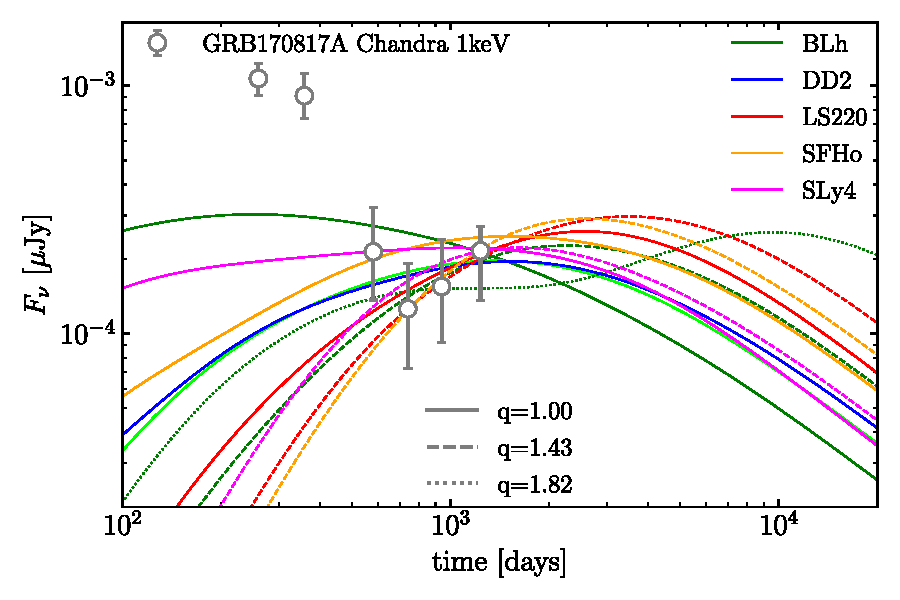
\includegraphics[height=5.0cm]{kn_afterglow/best_xray_obs_representative_all_eos.pdf}
%            %            Bolometric kN light curves in three representative bands from blue to
%            %            infrared for the two simulations with turbulence viscosity compared to
%            %            \AT{} data from~\citep{Villar:2017wcc}.
%            %            The color gradient is the effect related to different
%            %            \ac{SWW} masses, that suggests possible variations of the light
%            %            curves for different \ac{BNS}. The band is computed by extracting the
%            %            \ac{SWW} mass from DD2 every $10$~ms until the end of the simulation, and
%            %            then by linearly extrapolating the data to $250$~ms.
%            %            (Adapted from \citet{Nedora:2019jhl})
%    }};
%}
%
%Low opacity, fast \ac{SWW} 
%\uncover<1->{ % <-> |
%    \node (t2) [anchor=center,scale=1,opacity=1] at ([shift={(-3.8cm,-1.8cm)}]current page.center){
%        \parbox{0.6\textwidth}{
%            \begin{itemize}
%            \item Kilonova afterglow is consistent with rebrightneing of \GW{}
%            \item Models with $q>1$ and moderately soft \ac{EOS} fit better
%            \end{itemize}
%    }};
%}
%
%\end{tikzpicture}
%
%\end{frame}


%% =======================================================
%%
%%                   Result
%%
%% =======================================================

\begin{frame}{Kilonova afterglow for \GRB{} rebrightening} %% ---------- title 

\begin{tikzpicture}[overlay,remember picture]

\uncover<1->{ % <-> |
    \node (t1) [anchor=center,scale=1,opacity=1] at ([shift={(-0.8cm,1.8cm)}]current page.center){
        \parbox{1.0\textwidth}{
            \begin{itemize}
            \item Kilonova afterglow is consistent with rebrightneing of \GW{}
            \item Models with $q>1$ and moderately soft \ac{EOS} fit better
            \end{itemize}
    }};
}

\uncover<1->{ % <-> |
    \node (img1) [anchor=center,scale=1,opacity=1] at ([shift={(-4.0cm,-1.5cm)}]current page.center){
        \parbox{0.5\textwidth}{
            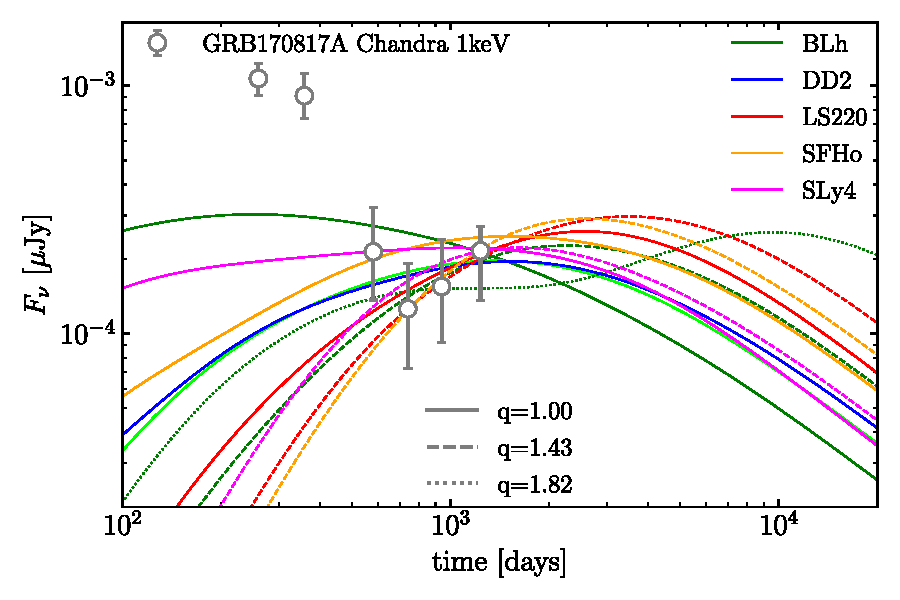
\includegraphics[height=5cm]{kn_afterglow/best_xray_obs_representative_all_eos.pdf}
    }};
}

\uncover<1->{ % <-> |
    \node (img1) [anchor=center,scale=1,opacity=1] at ([shift={(4.0cm,-1.5cm)}]current page.center){
        \parbox{0.5\textwidth}{
            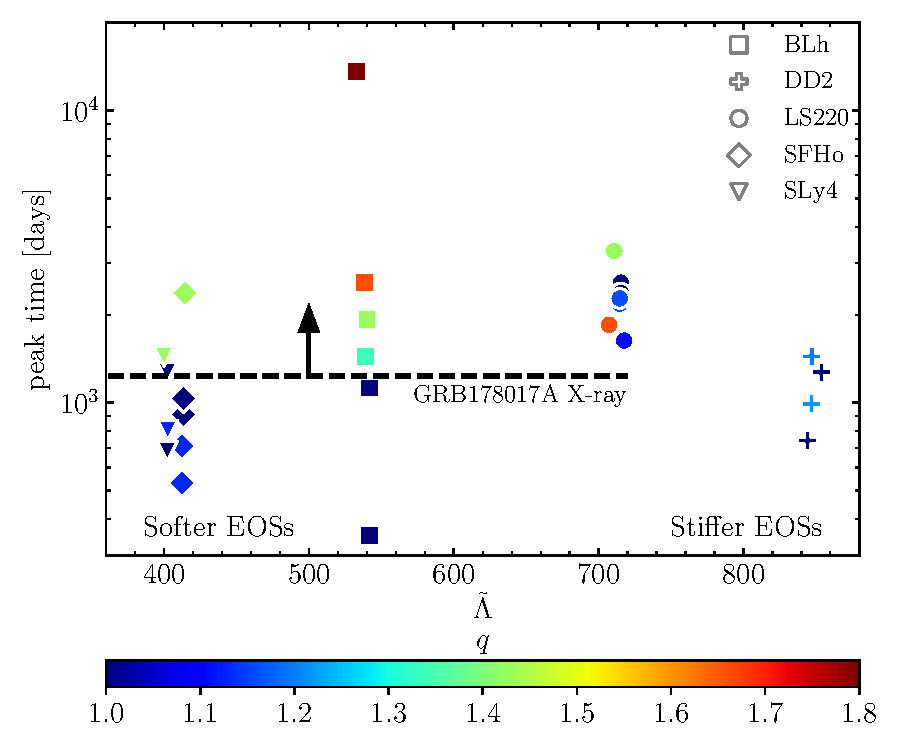
\includegraphics[height=5cm]{kn_afterglow/scatter_lightcurve_tpeak_vs_lambda.pdf}
    }};
}

\end{tikzpicture}

\end{frame}